\section*{Aufgabe 1: Zyklische Voltametrie (10)}
\begin{enumerate}
\item Zeichnen sie schematisch den \(H_{upd}\)-Bereich einer Pt-Polykristallelektrode
(\(0-0\, , 4\, V\,vs.\, RHG\)). (3)
\item Zeichnen sie den selben Bereich für eine Pt-Einkristallelektrode. (3)
\item Markieren sie im unten stehenden \(CO\)-Stripping-Diagramm den Bereich, den
sie zur Bestimmung der \textit{ECSA} verwenden und beschreiben sie ihr Vorgehen. (3)

\begin{center}
\begin{minipage}{\linewidth}
\centering
\makebox[0cm]{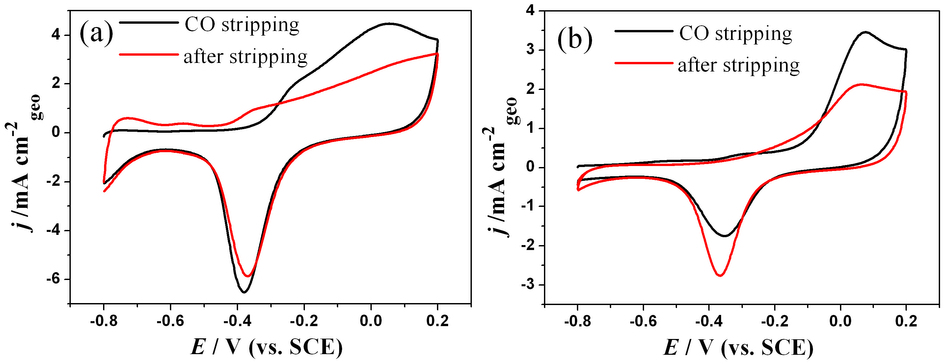
\includegraphics[width=10cm]{srep01181-f7.jpg}}
\captionof{figure}{Ungefähre Abbildung aus der Klausur}
\end{minipage}
\end{center}

\item Warum sind für den \(CO\)-Stripping Fall die Ungenauigkeiten bei der Bestimmung
der Oberfläche geringer als für die \(H_{upd}\)-Abschätzung? (1)

\end{enumerate}